\documentclass[aspectratio=169,10pt]{beamer}
\usepackage[utf8]{inputenc}
\usepackage[T1]{fontenc}
\usepackage[spanish,es-nodecimaldot]{babel}
\usepackage{lmodern}
\usepackage{graphicx}
\usepackage{booktabs}
\usepackage{array}
\usepackage{amsmath,amssymb}
\graphicspath{{figures/source/}{figures/adapted/}}
\newcommand{\DefenseTitle}{Reconstrucción de Canales EEG Faltantes Mediante Procesamiento de Señales en Grafos con Regularización Temporal}
\newcommand{\DefenseAuthor}{Carlos Saldivia Heinz}
\newcommand{\DefenseDegree}{Magíster en Ciencias de la Ingeniería}
\newcommand{\DefenseDepartment}{Departamento de Electrónica}
\newcommand{\DefenseInstitution}{Universidad Técnica Federico Santa María}
\newcommand{\DefenseAdvisor}{Profesor guía: Alejandro Weinstein, Ph.D.}
\newcommand{\DefenseDate}{Fecha de defensa: por definir}

\definecolor{USMBlue}{HTML}{004B76}
\definecolor{USMLight}{HTML}{EAF3F8}
\definecolor{USMGold}{HTML}{D9A441}
\definecolor{Ink}{HTML}{17242D}
\definecolor{Muted}{HTML}{5C6B73}
\definecolor{Good}{HTML}{1F7A5A}
\definecolor{Caution}{HTML}{A66518}
\definecolor{Bad}{HTML}{A63D40}

\setbeamercolor{normal text}{fg=Ink,bg=white}
\setbeamercolor{structure}{fg=USMBlue}
\setbeamercolor{frametitle}{fg=white,bg=USMBlue}
\setbeamercolor{title}{fg=white}
\setbeamercolor{subtitle}{fg=USMLight}
\setbeamercolor{author}{fg=white}
\setbeamercolor{institute}{fg=USMLight}
\setbeamercolor{date}{fg=USMLight}
\setbeamercolor{block title}{fg=white,bg=USMBlue}
\setbeamercolor{block body}{fg=Ink,bg=USMLight}
\setbeamercolor{alerted text}{fg=Bad}
\setbeamerfont{frametitle}{series=\bfseries,size=\Large}
\setbeamerfont{title}{series=\bfseries,size=\LARGE}
\setbeamerfont{subtitle}{size=\large}
\setbeamerfont{normal text}{size=\normalsize}
\setbeamertemplate{navigation symbols}{}
\setbeamertemplate{itemize item}{\color{USMGold}$\blacktriangleright$}
\setbeamertemplate{itemize subitem}{\color{USMBlue}$\bullet$}
\setbeamertemplate{frametitle}{\nointerlineskip\begin{beamercolorbox}[wd=\paperwidth,ht=0.82cm,dp=0.22cm,leftskip=0.46cm]{frametitle}\insertframetitle\end{beamercolorbox}}
\setbeamertemplate{footline}{%
  \leavevmode\hbox{%
  \begin{beamercolorbox}[wd=.80\paperwidth,ht=2.8ex,dp=1.1ex,leftskip=.45cm]{author in head/foot}\color{Muted}\scriptsize Carlos Saldivia Heinz · Defensa de título\end{beamercolorbox}%
  \begin{beamercolorbox}[wd=.20\paperwidth,ht=2.8ex,dp=1.1ex,rightskip=.45cm plus1fil]{date in head/foot}\color{USMBlue}\bfseries\scriptsize\insertframenumber\end{beamercolorbox}}}

% Keep source labels as normal UTF-8 text. Filename underscores are escaped at
% each call site so pdfLaTeX preserves both visual accents and searchable text.
\newcommand{\Source}[1]{\par\vspace{0.15em}{\color{Muted}\fontsize{6.2}{7.0}\selectfont Fuente: #1\par}}
\newcommand{\Takeaway}[1]{\begin{beamercolorbox}[rounded=true,sep=0.45em,wd=\linewidth]{block body}\centering\bfseries #1\end{beamercolorbox}}
\newcommand{\Metric}[3]{\begin{minipage}[t]{0.30\linewidth}\centering{\color{USMBlue}\fontsize{22}{24}\selectfont\bfseries #1}\par{\small #2}\par{\color{Muted}\scriptsize #3}\end{minipage}}
\newcommand{\SmallTag}[1]{\colorbox{USMLight}{\strut\scriptsize\bfseries\color{USMBlue}#1}}

% Valores congelados de la tesis para la defensa.
\newcommand{\MAEImprovement}{12{,}4\%}
\newcommand{\MAEInterval}{[+7{,}8; +17{,}4]\%}
\newcommand{\MAEWinRate}{72{,}0\%}
\newcommand{\NRMSEImprovement}{13{,}9\%}
\newcommand{\NRMSEWinRate}{70{,}3\%}
\newcommand{\DTWImprovement}{9{,}8\%}
\newcommand{\LSDImprovement}{-2{,}3\%}
\newcommand{\LSDWinRate}{40{,}7\%}
\newcommand{\MNETime}{0{,}0090~s/caso}
\newcommand{\TRSSTime}{0{,}1214~s/caso}
\newcommand{\FinalPairs}{300}
\newcommand{\FinalStrata}{100}

\title{\DefenseTitle}
\subtitle{Defensa de título · \DefenseDegree}
\author{\DefenseAuthor}
\institute{\DefenseDepartment\\\DefenseInstitution\\[0.35em]\DefenseAdvisor}
\date{\DefenseDate}

\begin{document}

% 1
{\setbeamertemplate{footline}{}\setbeamercolor{background canvas}{bg=USMBlue}
\begin{frame}[plain]
  \titlepage
  \vfill
  {\color{USMLight}\small Pregunta de apertura: ¿cuándo la continuidad temporal agrega información útil a una referencia espacial madura?}
  \vspace*{0.28cm}
\end{frame}}
\setcounter{framenumber}{0}

% 2
\begin{frame}{1. El problema real: un canal faltante altera lo que sigue}
\begin{columns}[T,onlytextwidth]
\column{0.56\textwidth}
\begin{block}{Cadena de impacto}
\centering
\Large Registro EEG $\longrightarrow$ canal ausente $\longrightarrow$ topografía incompleta\\[0.5em]
$\longrightarrow$ análisis temporal/espectral condicionado
\end{block}
\vspace{0.5em}
\begin{itemize}
\item Descartar ensayos reduce información disponible.
\item Sustituir el canal introduce una decisión metodológica.
\item La calidad debe medirse donde la señal verdadera es conocida.
\end{itemize}
\column{0.40\textwidth}
\Takeaway{Interpolar no es “rellenar”: es controlar cuánto sesgo se introduce antes del análisis.}
\vspace{0.7em}
\centering\SmallTag{Canales ocultos con verdad de terreno}
\end{columns}
\Source{Tesis, Introducción y Metodología, protocolo de ocultamiento artificial.}
\end{frame}

% 3
\begin{frame}{2. ¿Por qué interpolar EEG no es trivial?}
\begin{columns}[T,onlytextwidth]
\column{0.48\textwidth}
\begin{block}{Información espacial}
Electrodos cercanos suelen compartir estructura, pero una pérdida agrupada elimina vecinos informativos.
\end{block}
\begin{block}{Información temporal}
La señal evoluciona en el tiempo; regularizar demasiado puede suavizar componentes relevantes.
\end{block}
\column{0.48\textwidth}
\begin{block}{Múltiples criterios}
Menor error de amplitud no garantiza mejor preservación espectral ni menor costo.
\end{block}
\begin{block}{Consecuencia}
La elección depende del patrón de pérdida, la métrica y el uso posterior.
\end{block}
\end{columns}
\Source{Tesis, caps. 1, 2 y 5.}
\end{frame}

% 4
\begin{frame}{3. Brecha: no basta una línea base débil ni una métrica única}
\begin{columns}[T,onlytextwidth]
\column{0.31\textwidth}\begin{block}{Comparador}\centering Implementaciones propias pueden subestimar una referencia comunitaria madura.\end{block}
\column{0.31\textwidth}\begin{block}{Evaluación}\centering MAE por sí solo oculta tensiones de forma, espectro y tiempo.\end{block}
\column{0.31\textwidth}\begin{block}{Escenarios}\centering Pérdidas aleatorias simples no representan fallas localizadas y severas.\end{block}
\end{columns}
\vspace{0.7em}
\Takeaway{La tesis exige comparación fuerte, diseño pareado, múltiples regímenes y trazabilidad.}
\Source{Tesis, Introducción, sección “Brecha en la literatura”.}
\end{frame}

% 5
\begin{frame}{4. Preguntas y objetivo de la investigación}
\begin{block}{P1}
¿En qué condiciones la regularización espacio--temporal mejora la reconstrucción frente a métodos espaciales de referencia?
\end{block}
\begin{block}{P2}
¿Qué compromiso práctico existe entre precisión, fidelidad espectral y tiempo de cómputo al elegir entre TRSS y MNE-Python?
\end{block}
\vspace{0.25em}
\centering\textbf{Objetivo:} comparar estas dimensiones bajo un marco riguroso, reproducible y con variantes congeladas antes de la evaluación final.
\Source{Tesis, chapters/01\_introduccion.tex, líneas 40--67.}
\end{frame}

% 6
\begin{frame}{5. EEG como señal sobre un grafo}
\begin{columns}[T,onlytextwidth]
\column{0.76\textwidth}
\centering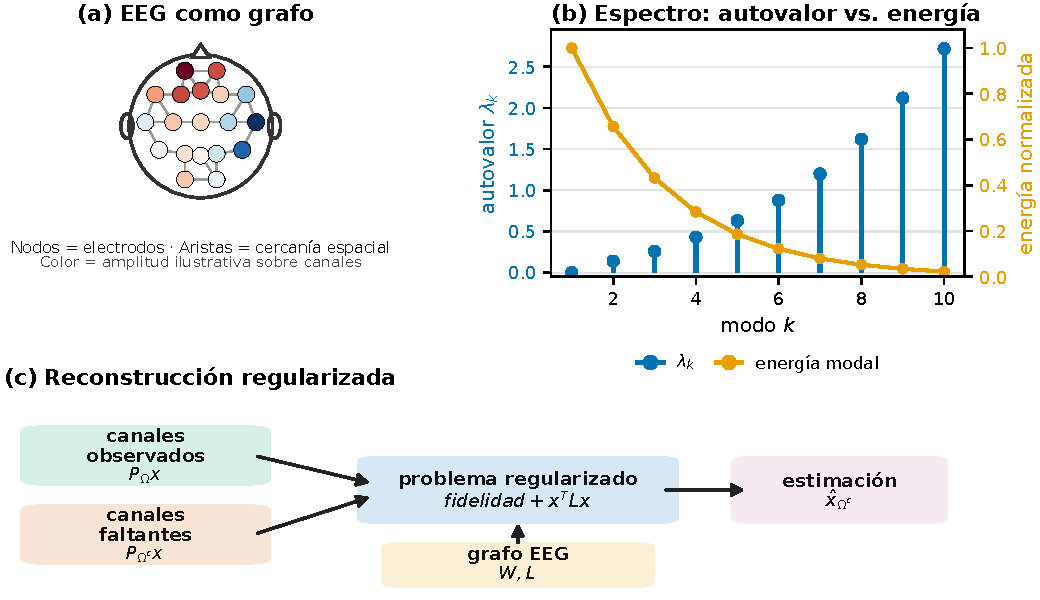
\includegraphics[width=0.98\linewidth,height=0.62\textheight,keepaspectratio]{ch2_gsp_concepts_clean.pdf}
\column{0.20\textwidth}
\raggedright\scriptsize
\begin{itemize}
\item Nodo: electrodo.
\item Arista: vecindad.
\item Peso: intensidad de relación.
\item Laplaciano: variación espacial.
\end{itemize}
\Takeaway{El grafo hace explícito qué canales pueden informar a uno faltante.}
\end{columns}
\Source{Tesis, cap. 2; figura ch2\_gsp\_concepts\_clean.pdf.}
\end{frame}

% 7
\begin{frame}{6. MNE frente a TRSS: dos fuentes de regularidad}
\begin{columns}[T,onlytextwidth]
\column{0.62\textwidth}
\centering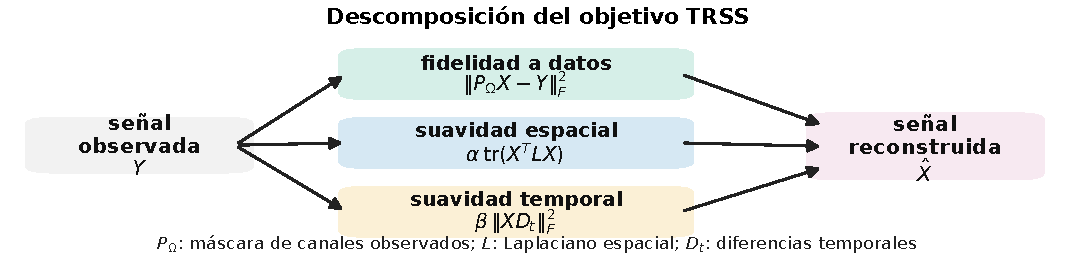
\includegraphics[width=\linewidth,height=0.65\textheight,keepaspectratio]{ch2_trss_operator.pdf}
\column{0.34\textwidth}
\begin{block}{MNE-Python}
Splines esféricos globales y una implementación comunitaria robusta.
\end{block}
\begin{block}{TRSS}
Fidelidad observada + suavidad espacial $\alpha$ + continuidad temporal $\beta$.
\end{block}
\end{columns}
\Source{Tesis, cap. 2; figura ch2\_trss\_operator.pdf.}
\end{frame}

% 8
\begin{frame}{7. Decisiones de alcance}
\small
\begin{tabular}{@{}>{\raggedright\arraybackslash}p{0.26\linewidth}>{\raggedright\arraybackslash}p{0.34\linewidth}>{\raggedright\arraybackslash}p{0.33\linewidth}@{}}
\toprule
\textbf{Decisión} & \textbf{Razón} & \textbf{Límite asumido}\\
\midrule
MNE-Python como referencia & Evitar un comparador debilitado & Resultado depende de versión/implementación\\
Grafos geométricos finales & Determinismo y ausencia de circularidad & Grafos aprendidos quedan abiertos\\
Sin modelos entrenables & No existía un protocolo externo de entrenamiento comparable & No se concluye contra toda alternativa futura\\
TRSS fijo como lectura principal & Parámetros congelados y reproducibles & Variante calibrada es auxiliar\\
\bottomrule
\end{tabular}
\vspace{0.5em}
\Takeaway{Las exclusiones protegen la interpretación; no son afirmaciones de imposibilidad.}
\Source{Tesis, Metodología y Discusión.}
\end{frame}

% 9
\begin{frame}{8. Estrategia experimental completa}
\centering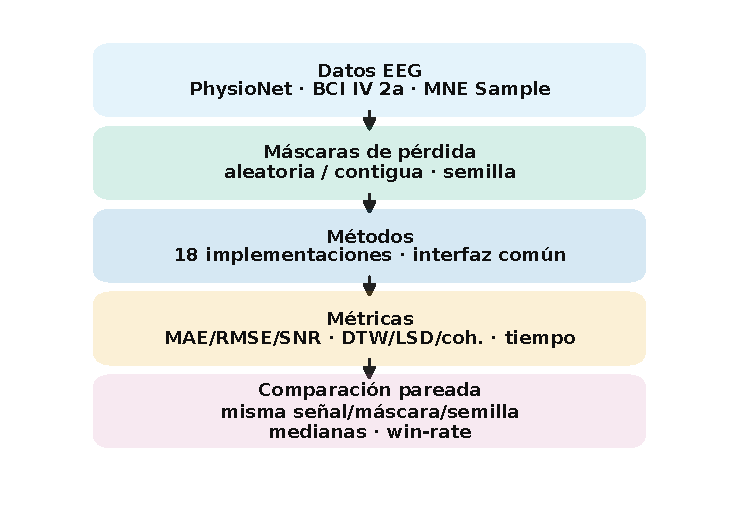
\includegraphics[width=0.92\linewidth,height=0.67\textheight,keepaspectratio]{ch3_methodology_flow.pdf}
\Takeaway{Explorar y seleccionar no es lo mismo que evaluar la comparación final.}
\Source{Tesis, figura ch3\_methodology\_flow.pdf.}
\end{frame}

% 10
\begin{frame}{9. Datos: diversidad sin prometer generalización poblacional}
\centering
\small
\begin{tabular}{@{}lrrrrl@{}}
\toprule
\textbf{Conjunto} & \textbf{Canales} & \textbf{Hz} & \textbf{Sujetos} & \textbf{Segmentos} & \textbf{Paradigma}\\
\midrule
PhysioNet & 64 & 160 & 109 & 60 s/sujeto & Reposo\\
BCI Competition IV 2a & 22 & 250 & 9 & 2.592 ensayos & Imaginación motora\\
MNE Sample & 60 & 600 & 1 & 72 ensayos & Auditivo\\
\bottomrule
\end{tabular}
\vspace{0.8em}
\begin{columns}[T,onlytextwidth]
\column{0.48\textwidth}\begin{block}{Aporta}Montajes, tasas de muestreo y paradigmas distintos.\end{block}
\column{0.48\textwidth}\begin{block}{No aporta}Una muestra representativa de toda población o uso clínico.\end{block}
\end{columns}
\Source{Tesis, Metodología, tabla de conjuntos de datos.}
\end{frame}

% 11
\begin{frame}{10. Cómo se simula la pérdida}
\begin{columns}[T,onlytextwidth]
\column{0.48\textwidth}
\begin{block}{Aleatoria}
Canales distribuidos al azar: aproxima fallas esporádicas.
\end{block}
\begin{block}{Contigua}
Canal semilla + vecinos cercanos: aproxima una falla localizada.
\end{block}
\column{0.48\textwidth}
\begin{block}{Fase amplia}
$3$ datasets $\times 2$ modos $\times 4$ severidades $\times 5$ semillas $=120$ escenarios.
\end{block}
\begin{block}{Control}
La misma máscara y semilla se entrega a todos los métodos.
\end{block}
\end{columns}
\vspace{0.4em}
\Takeaway{La verdad de terreno habilita error exacto, pero no reproduce toda falla real.}
\Source{Tesis, chapters/03\_metodologia.tex, líneas 35--41.}
\end{frame}

% 12
\begin{frame}{11. Evaluación multi-métrica: cada eje responde algo distinto}
\begin{columns}[T,onlytextwidth]
\column{0.23\textwidth}\begin{block}{Amplitud}\centering MAE\\RMSE/NRMSE\\SNR\end{block}
\column{0.23\textwidth}\begin{block}{Forma temporal}\centering DTW\\Correlación\\$R^2$\end{block}
\column{0.23\textwidth}\begin{block}{Espectro}\centering LSD\\Coherencia\\PSD\end{block}
\column{0.23\textwidth}\begin{block}{Costo}\centering Tiempo\\Complejidad\\Calibración\end{block}
\end{columns}
\vspace{0.8em}
\Takeaway{No se colapsan métricas incompatibles en un único “ganador”.}
\Source{Tesis, Metodología, sección Métricas; tabla ch6\_metric\_portfolio.tex.}
\end{frame}

% 13
\begin{frame}{12. Sistema experimental y trazabilidad}
\begin{columns}[T,onlytextwidth]
\column{0.69\textwidth}
\centering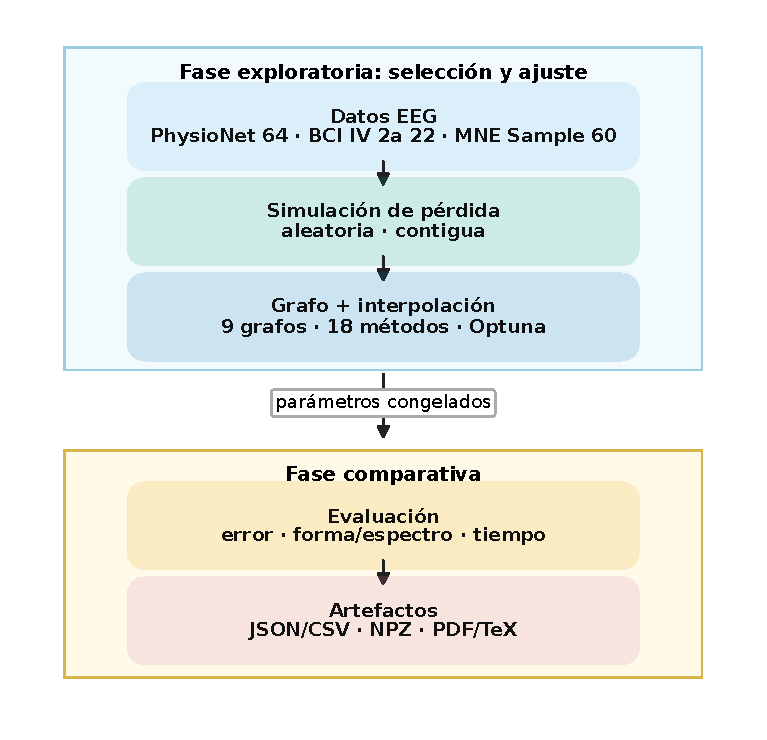
\includegraphics[width=\linewidth,height=0.66\textheight,keepaspectratio]{ch3_architecture_blocks.pdf}
\column{0.27\textwidth}
\begin{itemize}
\item Configuración inmutable.
\item Máscara y semilla.
\item Métricas y tiempos.
\item Señal reconstruida.
\item Identificador SHA-256.
\end{itemize}
\end{columns}
\Source{Tesis, Metodología; figura ch3\_architecture\_blocks.pdf.}
\end{frame}

% 14
\begin{frame}{13. De 18 métodos a una comparación defendible}
\centering
\begin{beamercolorbox}[rounded=true,sep=0.6em,wd=0.90\linewidth]{block body}
\centering\Large
18 métodos + 9 grafos\\[0.35em]
$\Downarrow$ \small selección preliminar\\[0.35em]
$\Downarrow$ \small descarte por inestabilidad, costo o circularidad\\[0.35em]
$\Downarrow$ \small optimización y congelamiento\\[0.35em]
$\Downarrow$ \Large TRSS fijo frente a MNE-Python
\end{beamercolorbox}
\vspace{0.6em}
\begin{alertblock}{Separación clave}
La fase amplia orienta decisiones. Solo el protocolo final congelado sostiene las cifras centrales.
\end{alertblock}
\Source{Tesis, tablas ch4\_experimental\_phase\_overview.tex y ch4\_candidate\_reduction\_decisions.tex.}
\end{frame}

% 15
\begin{frame}{14. Protocolo final: comparación pareada y congelada}
\begin{columns}[T,onlytextwidth]
\column{0.58\textwidth}
\begin{block}{Cada par comparte}
\centering Señal $+$ máscara $+$ semilla $+$ preprocesamiento
\end{block}
\centering
{\large TRSS fijo $\longrightarrow$ $\Delta_i$ $\longleftarrow$ MNE-Python}\\[0.45em]
{\small $\Delta_i=q(\mathrm{TRSS}_i)-q(\mathrm{MNE}_i)$}\par
{\scriptsize $q$: métrica evaluada en el mismo caso $i$}
\column{0.38\textwidth}
\centering
{\color{USMBlue}\LARGE\bfseries \FinalStrata\ $\times$ 3}\par {\small estratos $\times$ semillas}\par {\scriptsize régimen $\times$ patrón $\times$ severidad}\par\vspace{0.7em}
{\color{USMBlue}\LARGE\bfseries $=$ \FinalPairs}\par {\small diferencias pareadas}\par {\scriptsize no 300 sujetos independientes}\par\vspace{0.7em}
{\color{USMBlue}\LARGE\bfseries 1.000}\par {\small remuestreos}\par {\scriptsize bootstrap jerárquico descriptivo}
\end{columns}
\vspace{0.35em}
\Takeaway{Unidad observacional: $\Delta$ por estrato $\times$ semilla ($n=300$); unidad de agrupación: estrato ($n=100$).}
\Source{Tesis, Metodología, Protocolo de Validación Comparativa.}
\end{frame}

% 16
\begin{frame}{15. Resultado principal: ventaja descriptiva en MAE}
\begin{columns}[T,onlytextwidth]
\column{0.66\textwidth}
\centering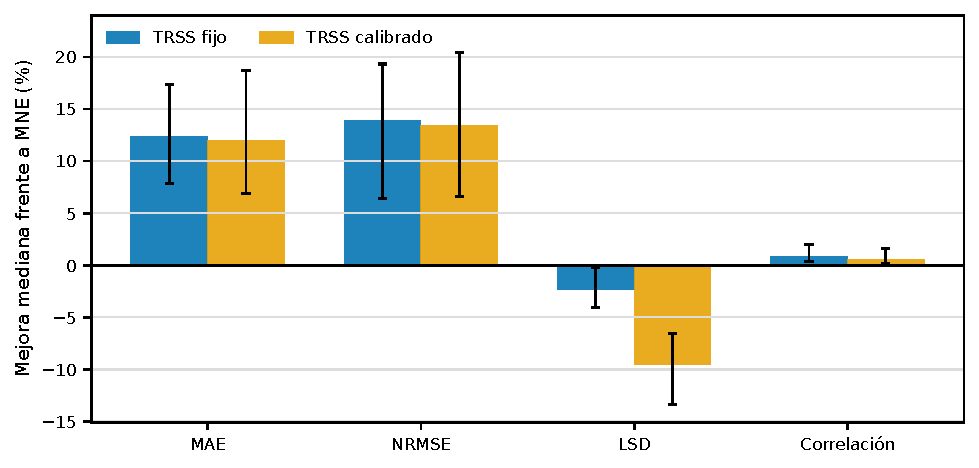
\includegraphics[width=\linewidth,height=0.66\textheight,keepaspectratio]{ch6_robust_improvement_ci.pdf}
\column{0.30\textwidth}
\centering
{\color{Good}\fontsize{26}{28}\selectfont\bfseries +\MAEImprovement}\par
{\small mejora mediana}\par\vspace{0.5em}
{\bfseries \MAEInterval}\par{\scriptsize IC descriptivo 95\%}\par\vspace{0.7em}
{\color{USMBlue}\fontsize{24}{26}\selectfont\bfseries \MAEWinRate}\par{\small victorias}
\end{columns}
\Source{Tesis, ch6\_robust\_main.tex; figura ch6\_robust\_improvement\_ci.pdf.}
\end{frame}

% 17
\begin{frame}{16. No hay un ganador universal}
\begin{columns}[T,onlytextwidth]
\column{0.76\textwidth}
\centering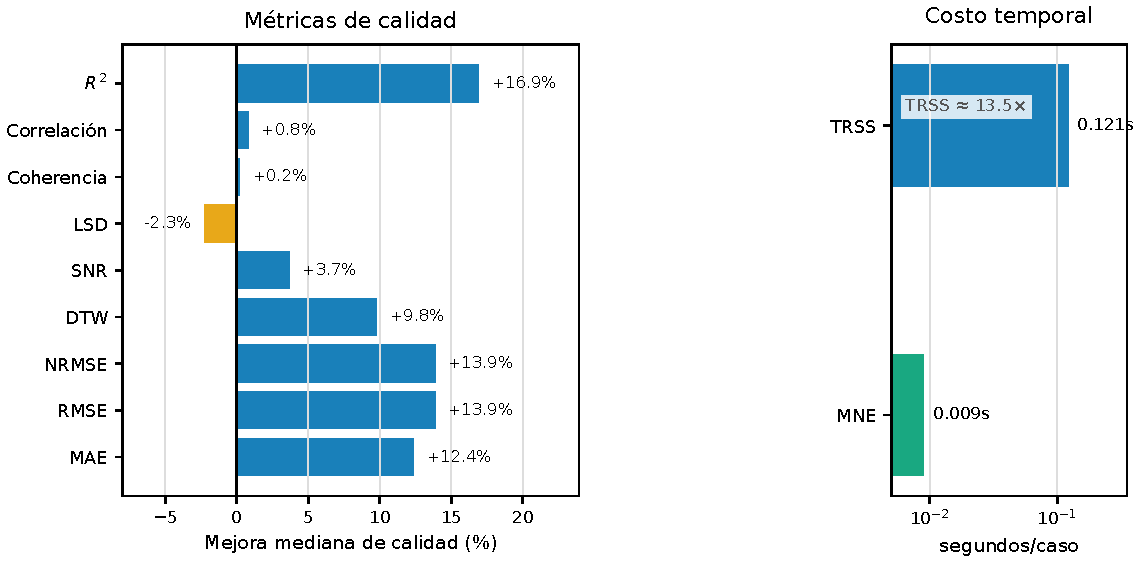
\includegraphics[width=\linewidth,height=0.63\textheight,keepaspectratio]{ch6_metric_portfolio_improvement.pdf}\\[-0.2em]
{\scriptsize Mejora relativa de TRSS frente a MNE; valores positivos favorecen a TRSS.}
\column{0.20\textwidth}
\raggedright\small
\begin{block}{Priorizar TRSS}
MAE, NRMSE, DTW, SNR y correlación.
\end{block}
\begin{block}{Priorizar MNE}
LSD global y tiempo: $\approx 13{,}5\times$ más rápido.
\end{block}
\end{columns}
\Source{Tesis, ch6\_metric\_portfolio.tex; figura ch6\_metric\_portfolio\_improvement.pdf.}
\end{frame}

% 18
\begin{frame}{17. ¿Cuándo ayuda TRSS? La ventaja es heterogénea}
\begin{columns}[T,onlytextwidth]
\column{0.79\textwidth}
\centering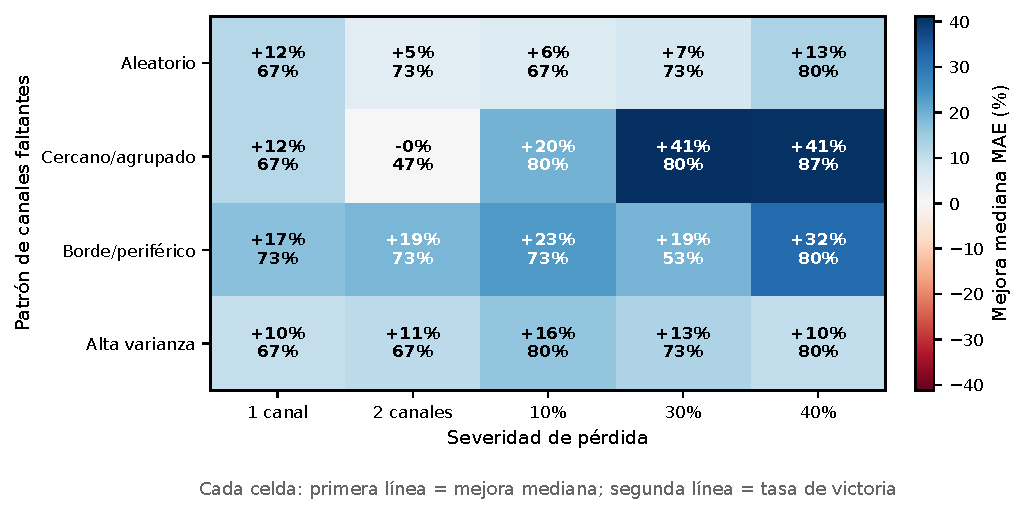
\includegraphics[width=\linewidth,height=0.70\textheight,keepaspectratio]{ch6_scenario_heatmap_mae.pdf}
\column{0.17\textwidth}
\raggedright\small
\begin{block}{Máximo}
\textbf{$+41\%$} en pérdida agrupada de 30--40\%; victorias: 80--87\%.
\end{block}
\begin{block}{Frontera}
\textbf{$\approx0\%$} con dos canales agrupados; victorias: 47\%.
\end{block}
\end{columns}
\Source{Tesis, ch6\_selected\_scenarios\_mae.tex; figura ch6\_scenario\_heatmap\_mae.pdf.}
\end{frame}

% 19
\begin{frame}{18. Qué ocurre en la señal: casos, no prueba global}
\centering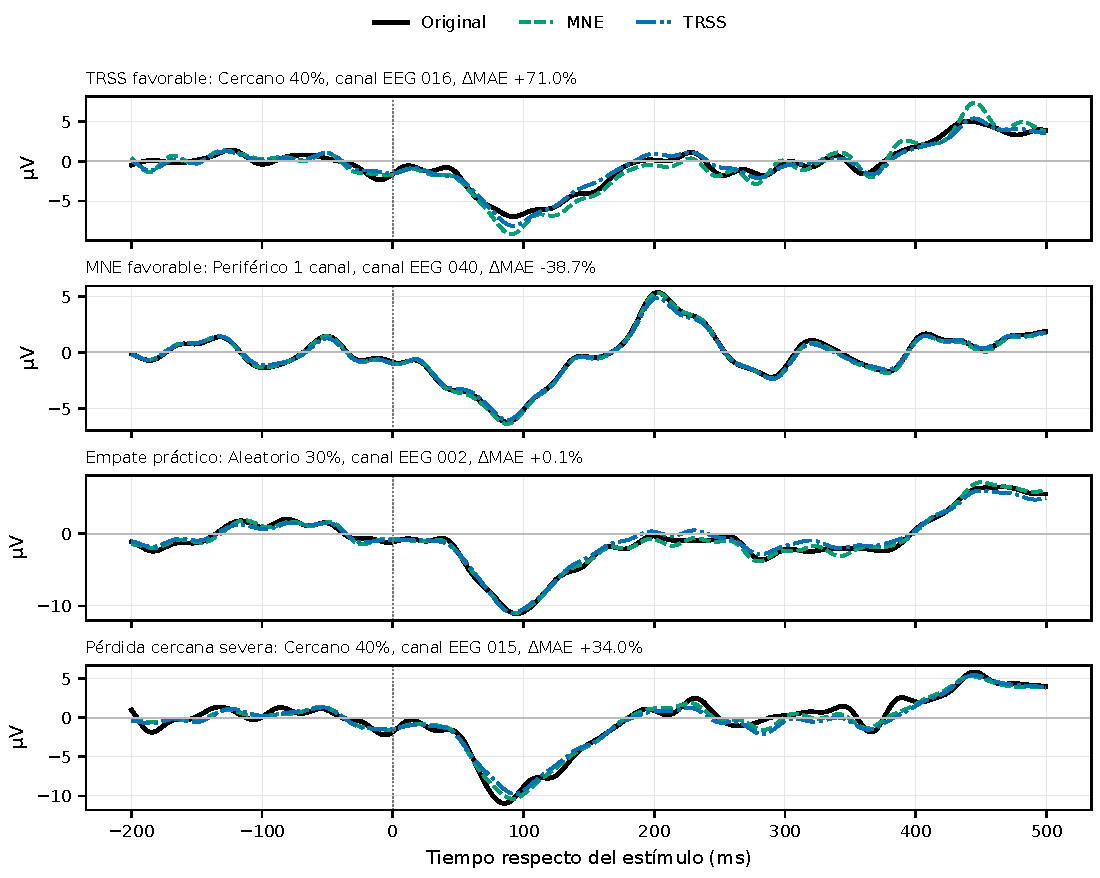
\includegraphics[width=0.95\linewidth,height=0.62\textheight,keepaspectratio]{ch4_representative_timeseries.pdf}
\Takeaway{Hay casos favorables a TRSS, favorables a MNE y empates; el agregado cuantitativo decide la tendencia.}
\Source{Tesis, Resultados; figura ch4\_representative\_timeseries.pdf.}
\end{frame}

% 20
\begin{frame}{19. Tensión espectral: menor MAE no implica menor LSD}
\begin{columns}[T,onlytextwidth]
\column{0.72\textwidth}
\centering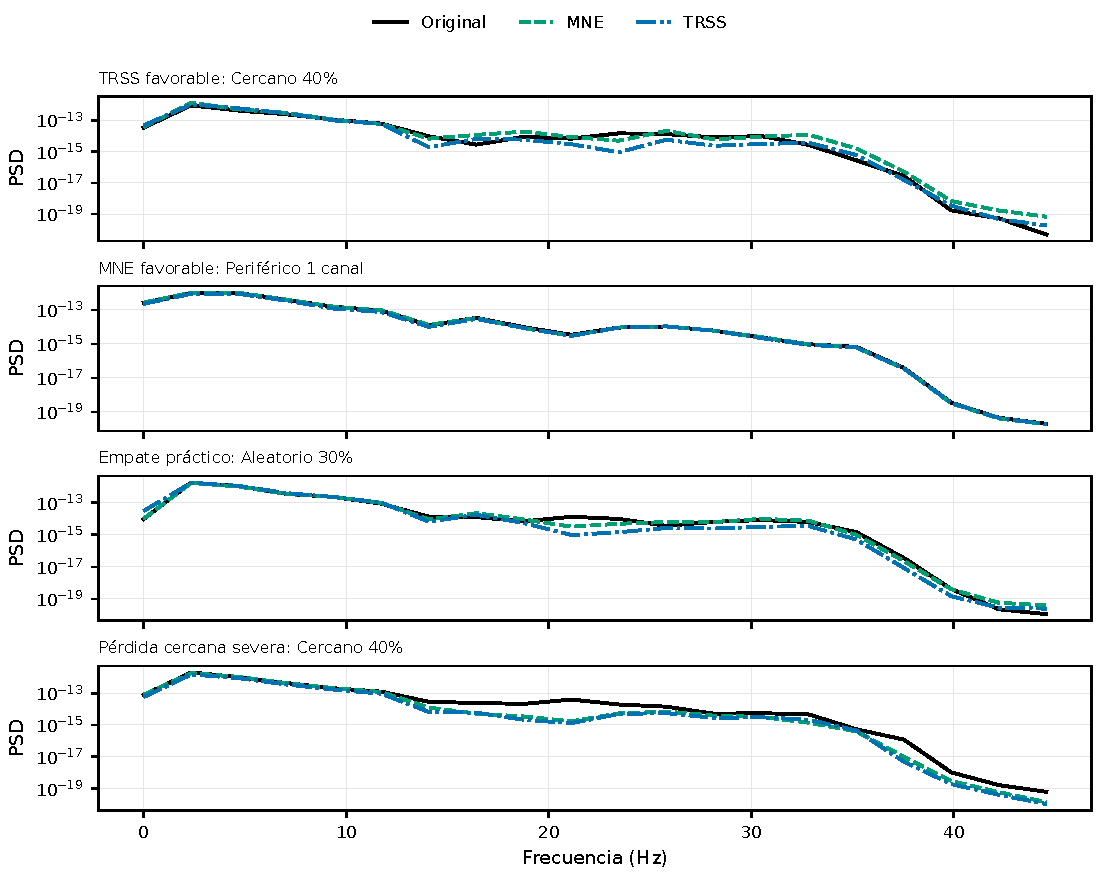
\includegraphics[width=\linewidth,height=0.67\textheight,keepaspectratio]{ch4_psd_original_vs_interpolated.pdf}
\column{0.24\textwidth}
\centering
{\color{Caution}\LARGE\bfseries \LSDImprovement}\par {\small LSD mediana}\par {\scriptsize favorece a MNE}\par\vspace{1.1em}
{\color{USMBlue}\LARGE\bfseries \LSDWinRate}\par {\small victorias TRSS}\par {\scriptsize en LSD}
\end{columns}
\Source{Tesis, Resultados y ch6\_metric\_portfolio.tex; figura de PSD.}
\end{frame}

% 21
\begin{frame}{20. Costo computacional: la ventaja de MNE es clara}
\begin{columns}[T,onlytextwidth]
\column{0.67\textwidth}
\centering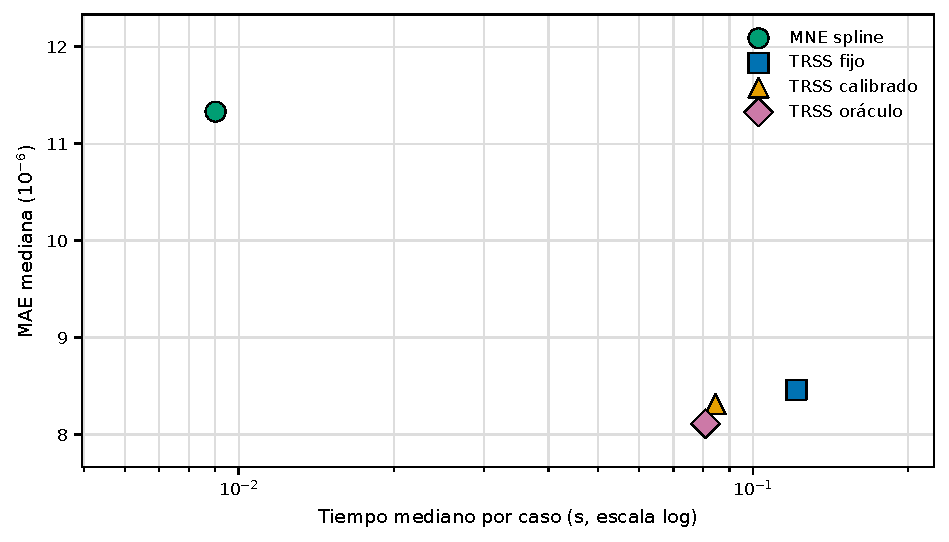
\includegraphics[width=\linewidth,height=0.65\textheight,keepaspectratio]{ch6_runtime_mae_tradeoff.pdf}
\column{0.29\textwidth}
\begin{block}{MNE-Python}\centering\Large\bfseries \MNETime\end{block}
\begin{block}{TRSS fijo}\centering\Large\bfseries \TRSSTime\end{block}
\small Medianas observadas; dependen de hardware, solver e implementación.
\end{columns}
\Source{Tesis, ch6\_runtime\_complexity.tex; figura ch6\_runtime\_mae\_tradeoff.pdf.}
\end{frame}

% 22
\begin{frame}{21. Frontera práctica de decisión}
\begin{columns}[T,onlytextwidth]
\column{0.66\textwidth}
\centering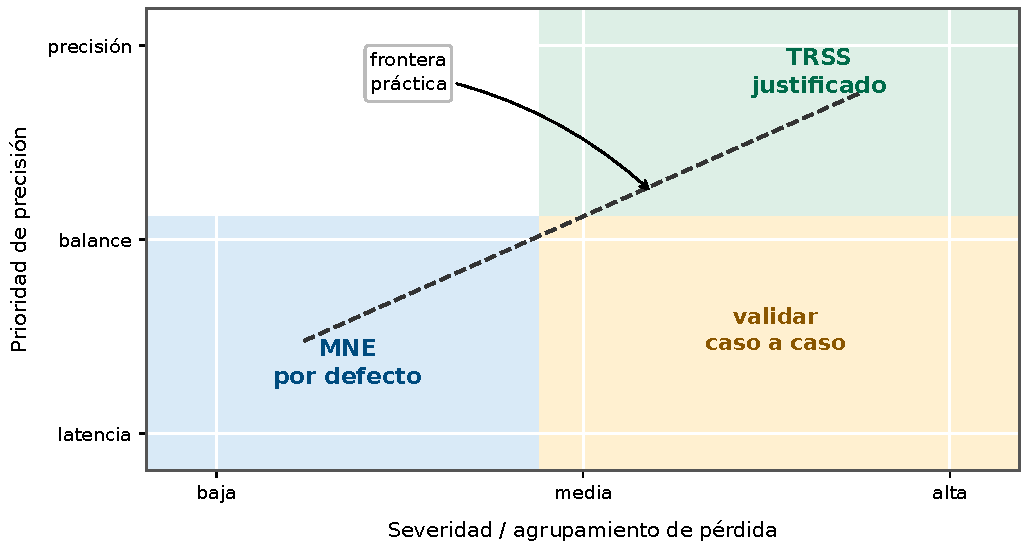
\includegraphics[width=\linewidth,height=0.66\textheight,keepaspectratio]{ch7_decision_map.pdf}
\column{0.30\textwidth}
\begin{block}{Preferir MNE}
Baja pérdida, prioridad espectral global, gran volumen o restricción de tiempo.
\end{block}
\begin{block}{Considerar TRSS}
Pérdida espacial difícil, análisis temporal fuera de línea y costo aceptable.
\end{block}
\end{columns}
\Source{Tesis, Discusión y Conclusiones; figura ch7\_decision\_map.pdf.}
\end{frame}

% 23
\begin{frame}{22. Aportes del trabajo}
\begin{columns}[T,onlytextwidth]
\column{0.48\textwidth}
\begin{block}{Científico}
Caracterización condicional de cuándo aporta regularización temporal.
\end{block}
\begin{block}{Metodológico}
Separación explícita entre exploración, reducción, congelamiento y evaluación.
\end{block}
\column{0.48\textwidth}
\begin{block}{Experimental}
Comparación pareada multi-métrica contra una referencia comunitaria fuerte.
\end{block}
\begin{block}{Reproducible}
Cadena trazable desde configuración y máscara hasta tabla, figura y afirmación.
\end{block}
\end{columns}
\Source{Tesis, Conclusiones, sección Aportes.}
\end{frame}

% 24
\begin{frame}{23. Limitaciones y fronteras de validez}
\small
\begin{tabular}{@{}>{\raggedright\arraybackslash}p{0.29\linewidth}>{\raggedright\arraybackslash}p{0.31\linewidth}>{\raggedright\arraybackslash}p{0.33\linewidth}@{}}
\toprule
\textbf{Límite} & \textbf{Qué permite afirmar} & \textbf{Qué falta}\\
\midrule
Ocultamiento artificial & Error con verdad de terreno & Canales realmente dañados\\
Medidas repetidas & Comparación pareada controlada & Generalización a nuevos sujetos/casos\\
Métricas de reconstrucción & Fidelidad en el benchmark & Impacto en tareas posteriores\\
Inspección visual y PSD & Coherencia cualitativa y espectral & Evaluación experta, ciega y protocolizada\\
Implementación observada & Costo relativo en este hardware & Optimización y validación de despliegue\\
\bottomrule
\end{tabular}
\vspace{0.7em}
\Takeaway{Evidencia válida bajo condiciones controladas; no se extrapola a daño real, nuevas poblaciones ni despliegue rutinario.}
\Source{Tesis, Discusión, “Deficiencias y carencias”; Conclusiones.}
\end{frame}

% 25
\begin{frame}{24. Conclusión: dos respuestas y una decisión}
\begin{block}{Respuesta a P1}
TRSS aporta valor en regímenes de pérdida espacial difícil, especialmente cuando faltan vecinos informativos; no reemplaza universalmente a MNE.
\end{block}
\begin{block}{Respuesta a P2}
La mejora en amplitud y forma temporal se intercambia por mayor costo y una desventaja en LSD global. La elección depende del objetivo.
\end{block}
\vspace{0.35em}
\Takeaway{El aporte central es identificar un régimen donde la temporalidad agrega información útil, documentar sus límites y dejar trazable el camino experimental.}
\vspace{0.35em}
\centering\small Futuro prioritario: acelerar TRSS · validar daño real y tareas posteriores · automatizar la decisión.
\Source{Tesis, Conclusiones, respuestas a P1/P2 y cierre.}
\end{frame}

% ---------------- BACKUP ----------------
\appendix
\begin{frame}{Respaldo B1. Formulación completa de TRSS}
\small
\[
\widehat{\mathbf X}=\arg\min_{\mathbf X}
\|\mathbf M\odot(\mathbf X-\mathbf Y)\|_F^2
+\alpha\,\mathrm{tr}(\mathbf X^\top\mathbf L\mathbf X)
+\beta\,\|\mathbf X\mathbf D_t\|_F^2
\]
\begin{itemize}
\item Primer término: fidelidad en canales observados.
\item $\alpha$: suavidad espacial sobre el Laplaciano del grafo.
\item $\beta$: continuidad temporal mediante diferencias finitas.
\item $\beta=0$: Tikhonov espacial independiente por instante.
\end{itemize}
\Source{Tesis, cap. 2, ecuación de TRSS.}
\end{frame}

\begin{frame}{Respaldo B2. Construcción del grafo k-NN gaussiano}
\[
W_{ij}=\exp\!\left(-\frac{\|\mathbf p_i-\mathbf p_j\|_2^2}{2\sigma^2}\right),\quad j\in\mathcal N_k(i)
\]
\begin{itemize}
\item $\mathbf p_i$: coordenada 3D del electrodo.
\item $k$: número de vecinos; $\sigma$: escala de decaimiento.
\item Determinista y construido sin usar la señal que luego se evalúa.
\item Grafos de correlación quedaron solo en exploración por circularidad potencial.
\end{itemize}
\Source{Tesis, caps. 2 y 3, construcción de grafos.}
\end{frame}

\begin{frame}{Respaldo B3. Spline propio no equivale a MNE-Python}
\small
\begin{tabular}{@{}>{\raggedright\arraybackslash}p{0.31\linewidth}>{\raggedright\arraybackslash}p{0.31\linewidth}>{\raggedright\arraybackslash}p{0.31\linewidth}@{}}
\toprule
& \textbf{Spline propio} & \textbf{MNE-Python}\\
\midrule
Objetivo & Referencia geométrica controlable & Herramienta comunitaria madura\\
Ingeniería & Implementación académica acotada & Normalización, restricciones, pseudoinversa, reintento\\
Uso final & Evidencia exploratoria & Comparador principal\\
Interpretación & No sustituye a MNE & Línea base fuerte\\
\bottomrule
\end{tabular}
\Source{Tesis, Introducción y Marco Teórico, mecanismo interno de MNE.}
\end{frame}

\begin{frame}{Respaldo B4. Familias exploradas}
\small
\begin{tabular}{@{}lp{0.67\linewidth}@{}}
\toprule
\textbf{Familia} & \textbf{Implementaciones representativas}\\
\midrule
Geométrica & Vecino más cercano, IDW, RBF, splines, lineal\\
Estadística & ICA/FastICA, ICA-MNE/Picard\\
GSP & Tikhonov, banda limitada, suavizado, TV, GTT\\
Espacio--temporal & TRSS y variantes\\
Referencia & MNE-Python por defecto y optimizada\\
\bottomrule
\end{tabular}
\vspace{0.5em}
Total declarado por la tesis: 18 implementaciones; solo TRSS y MNE avanzan a la comparación final.
\Source{Tesis, Metodología, tabla de métodos.}
\end{frame}

\begin{frame}{Respaldo B5. Optimización y congelamiento}
\small
\begin{tabular}{@{}lccc@{}}
\toprule
\textbf{Familia} & \textbf{Parámetros} & \textbf{Escala} & \textbf{Estrategia}\\
\midrule
GSP/grafo & $\sigma$, $k$ & Lineal & TPE, 30 intentos\\
TRSS & $\alpha$, $\beta$ & Log & Grilla fina\\
Splines propios & $m$, $\lambda$ & Mixta & NSGA-II, 10 intentos\\
MNE optimizada & $m$, $\lambda$ & Mixta & NSGA-II, 10 intentos\\
\bottomrule
\end{tabular}
\vspace{0.6em}
\begin{alertblock}{Regla}
TRSS fijo se congela antes del protocolo final. El oráculo es una cota no desplegable, no el resultado principal.
\end{alertblock}
\Source{Tesis, Metodología y tabla ch4\_intermediate\_optimization\_summary.tex.}
\end{frame}

\begin{frame}{Respaldo B6. Datasets, preprocesamiento y máscaras}
\small
\begin{itemize}
\item Preprocesamiento controlado: filtro Butterworth 0,5--45 Hz, referencia promedio común y segmentación uniforme.
\item Variables independientes: método, dataset, patrón, severidad y semilla.
\item Variables dependientes: métricas de amplitud, forma, espectro y costo.
\item Máscaras idénticas entre métodos; validadores comprueban correspondencia con la semilla.
\item Hardware reportado: Intel Core i7-13700H, 32 GB RAM, sin GPU.
\end{itemize}
\Source{Tesis, Metodología, Diseño Experimental y Control de Calidad.}
\end{frame}

\begin{frame}{Respaldo B7. Definición y dirección de métricas}
\small
\begin{tabular}{@{}lll@{}}
\toprule
\textbf{Dimensión} & \textbf{Métricas} & \textbf{Dirección favorable}\\
\midrule
Amplitud & MAE, RMSE, NRMSE & Menor\\
Relación señal--error & SNR & Mayor\\
Forma temporal & DTW, correlación, $R^2$ & Menor DTW; mayor correlación/$R^2$\\
Espectro & LSD, coherencia & Menor LSD; mayor coherencia\\
Costo & Tiempo por caso & Menor\\
\bottomrule
\end{tabular}
\vspace{0.6em}
La mejora porcentual se orienta para que valores positivos favorezcan a TRSS; en tiempo y LSD, los valores agregados negativos favorecen a MNE.
\Source{Tesis, Metodología y ch6\_metric\_portfolio.tex.}
\end{frame}

\begin{frame}{Respaldo B8. Bootstrap jerárquico y unidad estadística}
\begin{block}{Estructura}
300 pares anidados en 100 estratos; tres semillas por estrato; cada par comparte señal y máscara.
\end{block}
\begin{block}{Resumen}
Diferencias pareadas $\rightarrow$ mediana por estrato $\rightarrow$ remuestreo jerárquico de estratos y casos, 1.000 veces.
\end{block}
\begin{alertblock}{Interpretación}
Los intervalos describen estabilidad bajo el protocolo. No son p-valores ni convierten máscaras repetidas en sujetos independientes.
\end{alertblock}
\Source{Tesis, Metodología, Protocolo de Validación Comparativa.}
\end{frame}

\begin{frame}{Respaldo B9. Tabla numérica completa TRSS fijo–MNE}
\scriptsize
\begin{tabular}{@{}lrrr@{}}
\toprule
\textbf{Métrica} & \textbf{Mejora mediana} & \textbf{IC descriptivo 95\%} & \textbf{Victoria TRSS}\\
\midrule
MAE & +12,4\% & [+7,8; +17,4]\% & 72,0\%\\
NRMSE & +13,9\% & [+6,4; +19,3]\% & 70,3\%\\
DTW & +9,8\% & [+5,5; +12,7]\% & 71,0\%\\
SNR & +3,7\% & [+0,9; +9,6]\% & 61,0\%\\
LSD & -2,3\% & [-4,0; -0,2]\% & 40,7\%\\
Coherencia & +0,2\% & [0,0; +0,5]\% & 58,3\%\\
Correlación & +0,8\% & [+0,3; +2,0]\% & 68,7\%\\
$R^2$ & +16,9\% & [+3,4; +52,8]\% & 70,3\%\\
Tiempo & -1004,1\% & [-1072,8; -934,0]\% & 0,3\%\\
\bottomrule
\end{tabular}
\Source{Tesis, tables/ch6\_metric\_portfolio.tex.}
\end{frame}

\begin{frame}{Respaldo B10. Escenarios frontera en MAE}
\small
\begin{tabular}{@{}lrrr@{}}
\toprule
\textbf{Escenario} & \textbf{$n$} & \textbf{Victoria} & \textbf{Mejora}\\
\midrule
Cercano/agrupado, 40\% & 15 & 86,7\% & +40,8\%\\
Cercano/agrupado, 30\% & 15 & 80,0\% & +41,2\%\\
Borde/periférico, 40\% & 15 & 80,0\% & +31,6\%\\
Aleatorio, 40\% & 15 & 80,0\% & +13,0\%\\
Cercano/agrupado, 2 canales & 15 & 46,7\% & 0,0\%\\
\bottomrule
\end{tabular}
\vspace{0.5em}
Estas filas se usan para mostrar heterogeneidad; no son una estimación de prevalencia poblacional.
\Source{Tesis, ch6\_selected\_scenarios\_mae.tex.}
\end{frame}

\begin{frame}{Respaldo B11. Complejidad y costo de calibración}
\small
\begin{tabular}{@{}p{0.22\linewidth}p{0.46\linewidth}p{0.22\linewidth}@{}}
\toprule
\textbf{Método} & \textbf{Complejidad orientativa} & \textbf{Mediana}\\
\midrule
MNE spline & $O(N^3)+O(NT)$ & 0,0090 s/caso\\
TRSS fijo & $O(K(ET+NT))$ & 0,1214 s/caso\\
TRSS calibrado & $O(HK(ET+NT))$ & 0,0845 s/caso\\
\bottomrule
\end{tabular}
\vspace{0.6em}
$N$: canales; $T$: muestras; $E$: aristas; $K$: iteraciones; $H$: configuraciones. El tiempo calibrado observado no incluye una regla universal ni elimina el costo de búsqueda.
\Source{Tesis, ch6\_runtime\_complexity.tex.}
\end{frame}

\begin{frame}{Respaldo B12. Cadena de trazabilidad}
\centering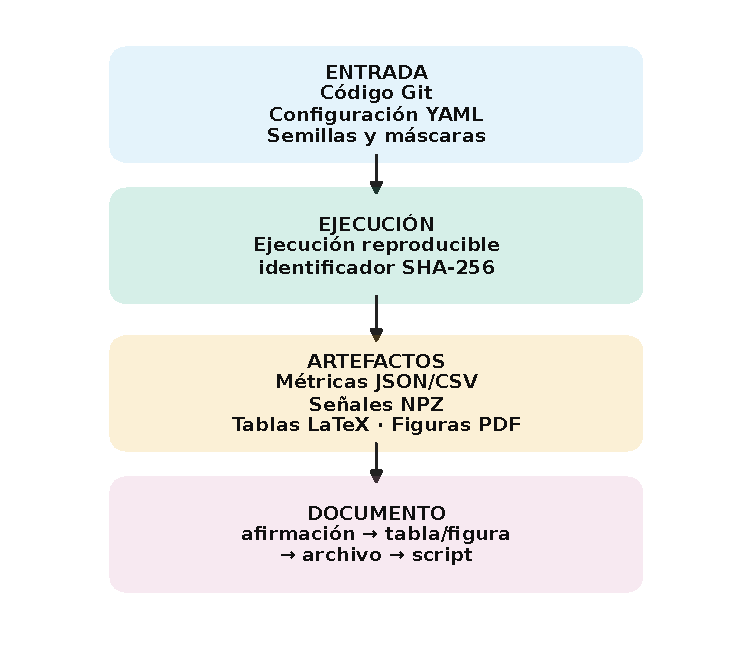
\includegraphics[width=0.90\linewidth,height=0.66\textheight,keepaspectratio]{ch4_traceability_pipeline.pdf}
\Takeaway{Afirmación $\rightarrow$ tabla/figura $\rightarrow$ resultado derivado $\rightarrow$ configuración, máscara y ejecución.}
\Source{Tesis, figura ch4\_traceability\_pipeline.pdf.}
\end{frame}

\begin{frame}{Respaldo B13. Validez: qué falta para ampliar el alcance}
\small
\begin{tabular}{@{}>{\raggedright\arraybackslash}p{0.22\linewidth}>{\raggedright\arraybackslash}p{0.33\linewidth}>{\raggedright\arraybackslash}p{0.36\linewidth}@{}}
\toprule
\textbf{Dimensión} & \textbf{Límite actual} & \textbf{Validación necesaria}\\
\midrule
Interna & Ocultamiento controlado, selección previa separada & Replicación y sensibilidad adicional\\
Constructo & Métricas proxy de reconstrucción & Evaluación ciega y tareas funcionales\\
Externa & Tres bases públicas y controles & Otros montajes, equipos y poblaciones\\
Práctica & Solver y hardware reportados & Optimización, memoria y latencia extremo a extremo\\
\bottomrule
\end{tabular}
\Source{Tesis, Discusión y Conclusiones.}
\end{frame}

\begin{frame}{Respaldo B14. Referencias principales}
\footnotesize
\begin{itemize}
\item Perrin et al. (1989). Spherical splines for scalp potential interpolation.
\item Shuman et al. (2013). The emerging field of signal processing on graphs.
\item Ortega et al. (2018). Graph signal processing: overview, challenges, applications.
\item Giraldo et al. (2022). Temporal regularization of graph signals / formulación TRSS usada por la tesis.
\item Gramfort et al. (2013, 2014). MNE software for processing electrophysiological data.
\item Akiba et al. (2019). Optuna: a next-generation hyperparameter optimization framework.
\end{itemize}
\vspace{0.5em}
Bibliografía completa y claves verificables en \texttt{references/references.bib} dentro de la tesis final.
\Source{Bibliografía de la tesis final.}
\end{frame}

\end{document}
